\documentclass[14pt]{extbook}
\usepackage{multicol, enumerate, enumitem, hyperref, color, soul, setspace, parskip, fancyhdr} %General Packages
\usepackage{amssymb, amsthm, amsmath, latexsym, units, mathtools} %Math Packages
\everymath{\displaystyle} %All math in Display Style
% Packages with additional options
\usepackage[headsep=0.5cm,headheight=12pt, left=1 in,right= 1 in,top= 1 in,bottom= 1 in]{geometry}
\usepackage[usenames,dvipsnames]{xcolor}
\usepackage{dashrule}  % Package to use the command below to create lines between items
\newcommand{\litem}[1]{\item#1\hspace*{-1cm}\rule{\textwidth}{0.4pt}}
\pagestyle{fancy}
\lhead{Progress Quiz 3}
\chead{}
\rhead{Version A}
\lfoot{3012-8528}
\cfoot{}
\rfoot{Summer C 2021}
\begin{document}

\begin{enumerate}
\litem{
Choose the equation of the function graphed below.
\begin{center}
    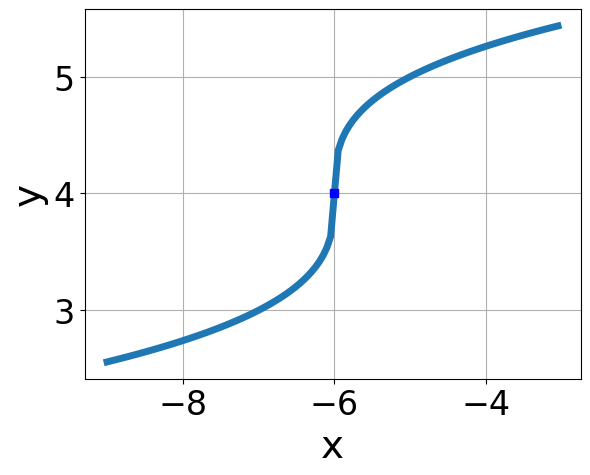
\includegraphics[width=0.5\textwidth]{../Figures/radicalGraphToEquationA.png}
\end{center}
\begin{enumerate}[label=\Alph*.]
\item \( f(x) = \sqrt[3]{x + 6} + 4 \)
\item \( f(x) = \sqrt[3]{x - 6} + 4 \)
\item \( f(x) = - \sqrt[3]{x - 6} + 4 \)
\item \( f(x) = - \sqrt[3]{x + 6} + 4 \)
\item \( \text{None of the above} \)

\end{enumerate} }
\litem{
What is the domain of the function below?\[ f(x) = \sqrt[4]{-7 x - 8} \]\begin{enumerate}[label=\Alph*.]
\item \( (-\infty, \infty) \)
\item \( [a, \infty), \text{where } a \in [-1.2, -1.07] \)
\item \( (-\infty, a], \text{where } a \in [-1.1, -0.39] \)
\item \( (-\infty, a], \text{ where } a \in [-1.24, -1.06] \)
\item \( [a, \infty), \text{where } a \in [-0.89, -0.69] \)

\end{enumerate} }
\litem{
Solve the radical equation below. Then, choose the interval(s) that the solution(s) belongs to.\[ \sqrt{-7 x - 6} - \sqrt{-4 x + 6} = 0 \]\begin{enumerate}[label=\Alph*.]
\item \( x_1 \in [-1.95, -0.73] \text{ and } x_2 \in [1.2,1.6] \)
\item \( \text{All solutions lead to invalid or complex values in the equation.} \)
\item \( x \in [-4.73,-3.97] \)
\item \( x_1 \in [-4.73, -3.97] \text{ and } x_2 \in [-3.2,0.8] \)
\item \( x \in [-0.65,0.93] \)

\end{enumerate} }
\litem{
Solve the radical equation below. Then, choose the interval(s) that the solution(s) belongs to.\[ \sqrt{-2 x + 6} - \sqrt{-3 x - 7} = 0 \]\begin{enumerate}[label=\Alph*.]
\item \( x \in [-16,-8] \)
\item \( \text{All solutions lead to invalid or complex values in the equation.} \)
\item \( x_1 \in [-5.33, -1.33] \text{ and } x_2 \in [1,5] \)
\item \( x_1 \in [-16, -8] \text{ and } x_2 \in [1,5] \)
\item \( x \in [0,4] \)

\end{enumerate} }
\litem{
Choose the equation of the function graphed below.
\begin{center}
    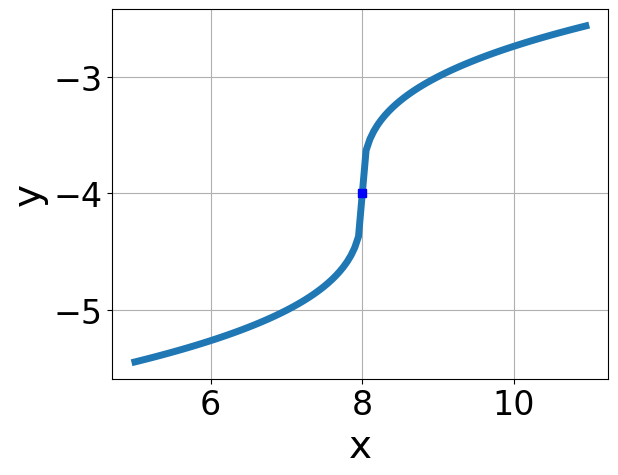
\includegraphics[width=0.5\textwidth]{../Figures/radicalGraphToEquationCopyA.png}
\end{center}
\begin{enumerate}[label=\Alph*.]
\item \( f(x) = \sqrt[3]{x - 8} - 4 \)
\item \( f(x) = - \sqrt[3]{x - 8} - 4 \)
\item \( f(x) = - \sqrt[3]{x + 8} - 4 \)
\item \( f(x) = \sqrt[3]{x + 8} - 4 \)
\item \( \text{None of the above} \)

\end{enumerate} }
\litem{
Solve the radical equation below. Then, choose the interval(s) that the solution(s) belongs to.\[ \sqrt{12 x^2 - 32} - \sqrt{8 x} = 0 \]\begin{enumerate}[label=\Alph*.]
\item \( x_1 \in [-1.73, -0.76] \text{ and } x_2 \in [0,6] \)
\item \( \text{All solutions lead to invalid or complex values in the equation.} \)
\item \( x_1 \in [0.82, 1.39] \text{ and } x_2 \in [0,6] \)
\item \( x \in [-1.73,-0.76] \)
\item \( x \in [1.89,2.04] \)

\end{enumerate} }
\litem{
Choose the graph of the equation below.\[ f(x) = - \sqrt[3]{x - 8} - 5 \]\begin{enumerate}[label=\Alph*.]
\begin{multicols}{2}\item 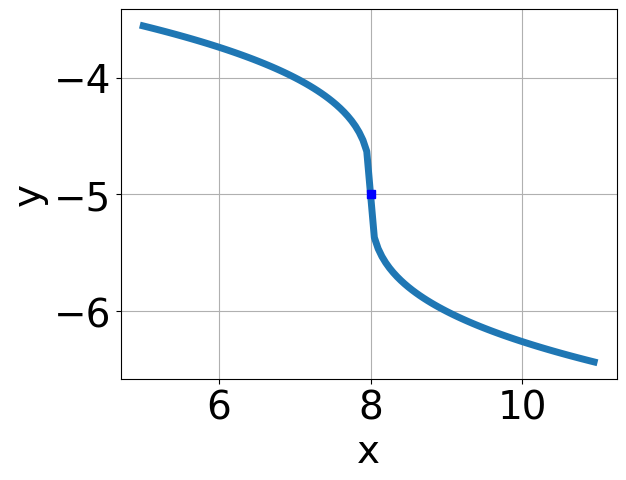
\includegraphics[width = 0.3\textwidth]{../Figures/radicalEquationToGraphAA.png}\item 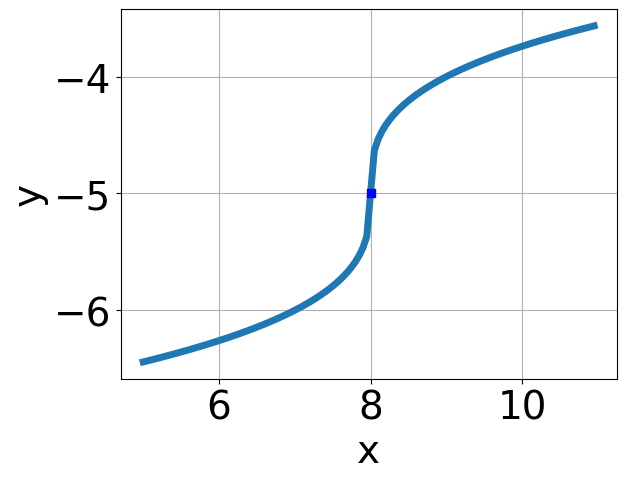
\includegraphics[width = 0.3\textwidth]{../Figures/radicalEquationToGraphBA.png}\item 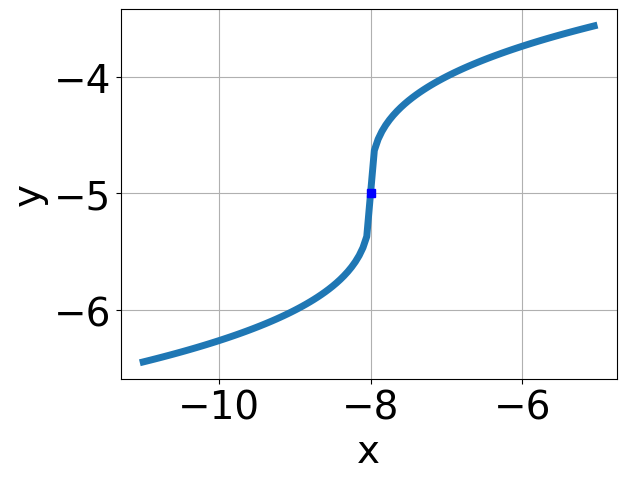
\includegraphics[width = 0.3\textwidth]{../Figures/radicalEquationToGraphCA.png}\item 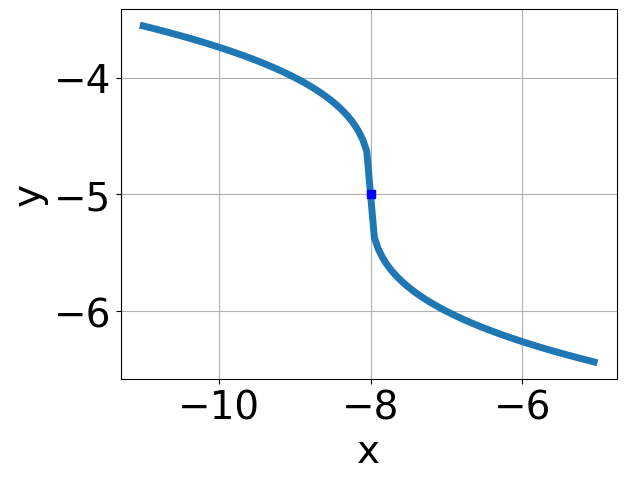
\includegraphics[width = 0.3\textwidth]{../Figures/radicalEquationToGraphDA.png}\end{multicols}\item None of the above.
\end{enumerate} }
\litem{
Solve the radical equation below. Then, choose the interval(s) that the solution(s) belongs to.\[ \sqrt{-27 x^2 + 35} - \sqrt{-24 x} = 0 \]\begin{enumerate}[label=\Alph*.]
\item \( x \in [1.6,2.1] \)
\item \( x_1 \in [-3.5, 0.1] \text{ and } x_2 \in [0.67,4.67] \)
\item \( \text{All solutions lead to invalid or complex values in the equation.} \)
\item \( x_1 \in [0.7, 1.4] \text{ and } x_2 \in [0.67,4.67] \)
\item \( x \in [-3.5,0.1] \)

\end{enumerate} }
\litem{
Choose the graph of the equation below.\[ f(x) = \sqrt{x - 12} - 3 \]\begin{enumerate}[label=\Alph*.]
\begin{multicols}{2}\item 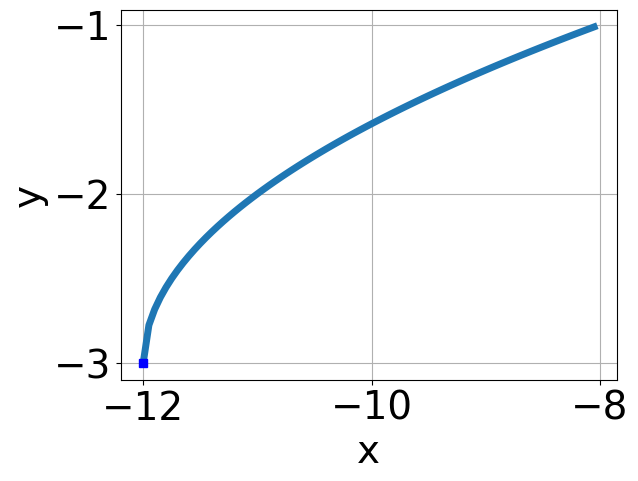
\includegraphics[width = 0.3\textwidth]{../Figures/radicalEquationToGraphCopyAA.png}\item 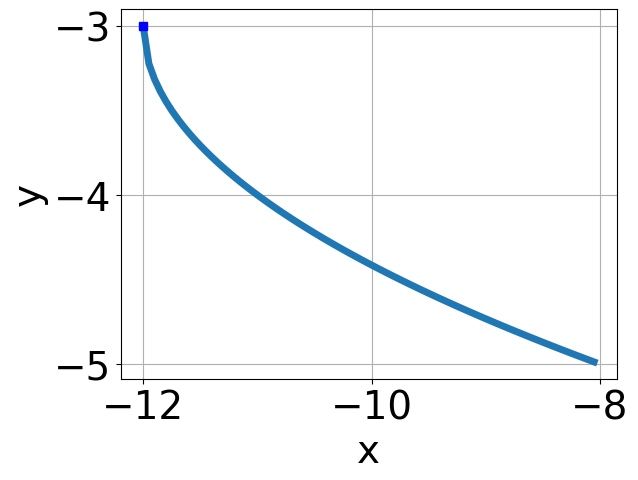
\includegraphics[width = 0.3\textwidth]{../Figures/radicalEquationToGraphCopyBA.png}\item 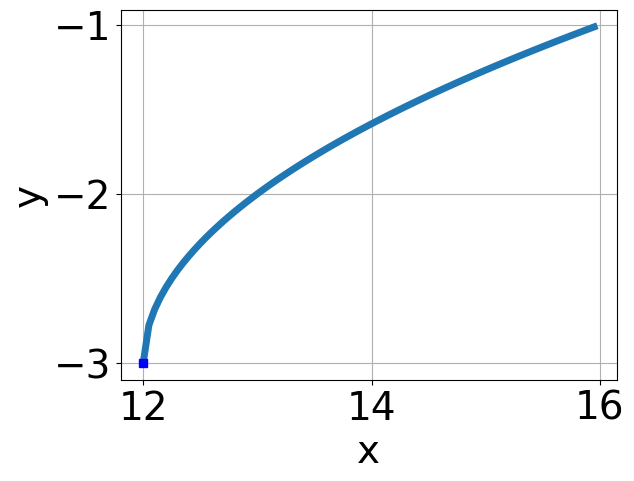
\includegraphics[width = 0.3\textwidth]{../Figures/radicalEquationToGraphCopyCA.png}\item 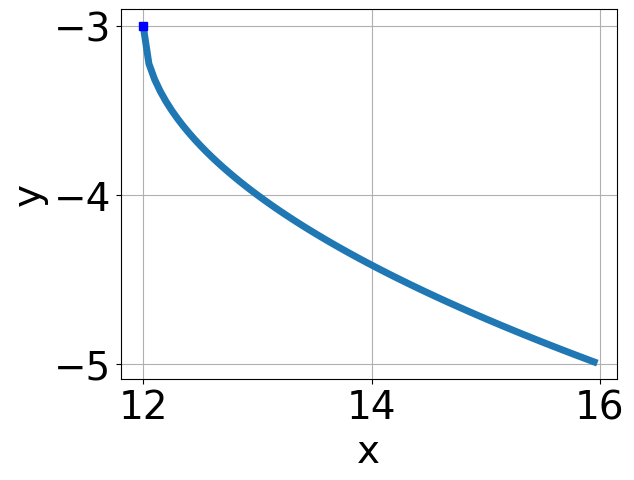
\includegraphics[width = 0.3\textwidth]{../Figures/radicalEquationToGraphCopyDA.png}\end{multicols}\item None of the above.
\end{enumerate} }
\litem{
What is the domain of the function below?\[ f(x) = \sqrt[3]{8 x + 9} \]\begin{enumerate}[label=\Alph*.]
\item \( \text{The domain is } (-\infty, a], \text{   where } a \in [-1.45, -1] \)
\item \( \text{The domain is } (-\infty, a], \text{   where } a \in [-0.96, -0.54] \)
\item \( (-\infty, \infty) \)
\item \( \text{The domain is } [a, \infty), \text{   where } a \in [-0.92, -0.86] \)
\item \( \text{The domain is } [a, \infty), \text{   where } a \in [-1.64, -1.01] \)

\end{enumerate} }
\end{enumerate}

\end{document}